%\documentclass[handout]{beamer}
\documentclass{beamer}
 
\usetheme[numbering = fraction, progressbar = none, background = light, sectionpage = progressbar]{metropolis}
\usepackage{multimedia}
\usepackage{amsmath}

\title{Econ 103 -- Statistics for Economists}
\subtitle{Intro and Chapter 1}
\author{Mallick Hossain}
\date{}
\institute{University of Pennsylvania}
\begin{document} 

%%%%%%%%%%%%%%%%%%%%%%%%%%%%%%%%%%%%%%%%
\begin{frame}
	\titlepage 
\end{frame} 

\section{Syllabus and Logistics}
%%%%%%%%%%%%%%%%%%%%%%%%%%%%%%%%%%%%%%%%
\begin{frame}
\frametitle{Where is Everything?}
	\begin{itemize}[<+- | alert@+>]
		\item  The Syllabus
		\item Course materials are on my website (\url{mallickhossain.com/econ-103})
		\item Grades are on Canvas (canvas.upenn.edu)
		\item Questions are on Piazza (piazza.com)
	\end{itemize}
\end{frame}

%%%%%%%%%%%%%%%%%%%%%%%%%%%%%%%%%%%%%%%%
\begin{frame}
\frametitle{Textbook}
	\begin{center}
		\includegraphics[scale=0.45]{./images/textbook.jpeg}
	\end{center}
	\centering
	Just get a used copy and save some money
\end{frame}

%%%%%%%%%%%%%%%%%%%%%%%%%%%%%%%%%%%%%%%%
\begin{frame}
\frametitle{Other Recommendations}
	\begin{center}
		\includegraphics[scale=0.45]{./images/How_to_Lie_with_Statistics.jpg}
	\end{center}
	\begin{center}
	Your ``Defense Against the Dark (Statistical) Arts'' guide. 100\% of teachers recommend it$^*$
	\end{center}
	\only<2->{\tiny{*based on a sample of Econ 103 teachers named Mallick Hossain ($n = 1$)}}
\end{frame}

%%%%%%%%%%%%%%%%%%%%%%%%%%%%%%%%%%%%%%%%
\begin{frame}
\frametitle{Other Recommendations}
	\begin{center}
		\includegraphics[scale=0.45]{./images/cartoon_stats.jpg}
	\end{center}
	\centering
	Everyone loves cartoons!\textsuperscript{\textcolor{blue}{[citation needed]}}
\end{frame}

%%%%%%%%%%%%%%%%%%%%%%%%%%%%%%%%%%%%%%%%
\begin{frame}
\frametitle{Grading}
	\begin{enumerate}
		\item \alert{Default Scheme}
			\begin{align*}
			\text{Final Grade} &= (20\% \times \text{R Project}) + (20\% \times \text{Midterm 1})  
			\\
			&+ (20\% \times \text{Midterm 2}) + (40\% \times \text{Final})
			\end{align*}
		\item \alert{Participation Scheme (must opt-in)}
			\begin{align*}
			\text{Final Grade} &= (15\% \times \text{Participation}) + (15\% \times \text{R Project})
			\\
			&+ (20\% \times \text{Midterm 1}) + (20\% \times \text{Midterm 2})
			\\
			&+ (30\% \times \text{Final})
			\end{align*}
	\end{enumerate}
\end{frame}

%%%%%%%%%%%%%%%%%%%%%%%%%%%%%%%%%%%%%%%%
\begin{frame}
\frametitle{Participation}
	\begin{itemize}
		\item Your participation grade will be based on the following:
			\begin{itemize}
				\item In-class participation
				\item Piazza participation
				\item Homework assignments
			\end{itemize}
	\end{itemize}
	\only<2->{\alert{In short, get involved in the course!}}
\end{frame}

%%%%%%%%%%%%%%%%%%%%%%%%%%%%%%%%%%%%%%%%
\begin{frame}
\frametitle{Attendance}
	\begin{itemize}
		\item I will not take attendance, so show up if it's helpful
		\item If you opted into the ``Participation'' grading scheme, part of your score comes from 			how active you are in class, so ask questions and \alert{\textsc{participate}}!
	\end{itemize}
\end{frame}

\section{R Project}
%%%%%%%%%%%%%%%%%%%%%%%%%%%%%%%%%%%%%%%%
\begin{frame}
\frametitle{Motivation}
    \begin{itemize}[<+- | alert@+>]
        \item Apply the skills and tools you have learned
        \item Answer questions you are interested in
        \item Head-start on honors thesis?
    \end{itemize}
\end{frame}

%%%%%%%%%%%%%%%%%%%%%%%%%%%%%%%%%%%%%%%%
\begin{frame}
\frametitle{What Subjects Can I Explore?}
    \begin{itemize}[<+- | alert@+>]
        \item ANYTHING\only<2->{, \alert<2>{seriously.}}
        \begin{itemize}
        		\item Political or ideological agendas are welcome
        		\item Guns, gender, inequality, race, climate change, \ldots
        		\item Google trends, Twitter, financial data, macro data, \ldots
        \end{itemize}
    \end{itemize}
\end{frame}

%%%%%%%%%%%%%%%%%%%%%%%%%%%%%%%%%%%%%%%%
\begin{frame}
\frametitle{What Do I Turn In?}
    \begin{itemize}[<+- | alert@+>]
        	\item Summary of question
		\item Summary of data and why it is relevant for the question			
		\item Tables and charts of summary stats of the data
		\item Data visualization/hypothesis testing
		\item Discussion of results
		\item Criticism of your findings. What are the biggest flaws in your analysis or in the underlying data?
		\item Suggestions for further analysis or extension to the project
    \end{itemize}
\end{frame}

%%%%%%%%%%%%%%%%%%%%%%%%%%%%%%%%%%%%%%%%
\begin{frame}
\frametitle{When is it Due?}
    \begin{itemize}
       \item \textbf{October 12:} Submit project idea and question or spoken with me about the project. Submit names of people in your group.

		\item \textbf{November 16:} (Optional) Submit rough draft for comments.

		\item \textbf{December 7:} Hand in project.
    \end{itemize}
\end{frame}

%%%%%%%%%%%%%%%%%%%%%%%%%%%%%%%%%%%%%%%%
\begin{frame}
\frametitle{Examples}
    \begin{itemize}[<+- | alert@+>]
        	\item R Tutorials provide examples of the kinds of exploration I am looking for
        	\item CEA blog posts on \href{https://www.whitehouse.gov/blog/2016/09/02/employment-situation-august}{jobs} and \href{https://www.whitehouse.gov/blog/2016/08/26/second-estimate-gross-domestic-product-second-quarter-2016}{GDP} and other publications (like the Economic Report of the President)
        	\item FiveThirtyEight's report on \href{http://fivethirtyeight.com/features/gun-deaths/}{gun deaths}
    \end{itemize}
\end{frame}

%%%%%%%%%%%%%%%%%%%%%%%%%%%%%%%%%%%%%%%%
\begin{frame}
\frametitle{Do I Need to Discover Something New?}
    \begin{itemize}[<+- | alert@+>]
        	\item Not looking for a Nobel-prize-winning discovery
        	\item You should learn something new
        	\item Hopefully I'll learn something new
        	\item Be honest
    \end{itemize}
\end{frame}

%%%%%%%%%%%%%%%%%%%%%%%%%%%%%%%%%%%%%%%%
\begin{frame}
\frametitle{How Do I Do Well In the Course?}
	\begin{itemize}[<+- | alert@+>]
		\item Don't cram
		\item Learn concepts, don't memorize
		\item Review slides shortly after lecture
		\item Quizzes assess your fundamental understanding
		\item Do the homework
		\item Learn R\alert<7>{\only<7>{, seriously.}}
	\end{itemize}
\end{frame}

%%%%%%%%%%%%%%%%%%%%%%%%%%%%%%%%%%%%%%%%
\begin{frame}
\frametitle{Learning Curves}
	There are two learning curves to be aware of in this course:
	\begin{enumerate}[<+- | alert@+>]
		\item \textbf{Statistics:} This will be a tough, but manageable one (like hiking up a constant moderate-graded mountain)
		\item \textbf{Statistical Programming:} This is probably best illustrated at the link below:
		\begin{itemize}
			\item \url{http://i.imgur.com/vPkUXWB.gif}
			\item The good news is that once you get around the curve, it will be a pleasant ride in a 			Cadillac
			\item Tutorials to make getting around the curve easier
		\end{itemize}
	\end{enumerate}
\end{frame}

%%%%%%%%%%%%%%%%%%%%%%%%%%%%%%%%%%%%%%%%
\begin{frame}
\frametitle{Course Outline}
	\begin{enumerate}[<+-|alert@+>]
		\item Descriptive Statistics: summarize data
			\begin{itemize}
				\item Summary Statistics and graphics
			\end{itemize}
		\item Probability: Population $\rightarrow$ Sample
			\begin{itemize}
				\item Deductive: ``safe'' argument
					\begin{itemize}
						\item All ducks waddle, swim, and quack. Donald is a duck. Donald must 								waddle, swim, and quack.
					\end{itemize}
			\end{itemize}
		\item Statistics: Sample $\rightarrow$ Population
			\begin{itemize}
				\item Inductive: ``risky'' argument
					\begin{itemize}
						\item If it walks like a duck, quacks like a duck, and swims like a duck, it's 							probably a duck
						\item When you hear hoofbeats, think horses, not zebras
					\end{itemize}
			 \end{itemize}
	\end{enumerate}
\end{frame}

\section{Motivation}
%%%%%%%%%%%%%%%%%%%%%%%%%%%%%%%%%%%%%%%%
\begin{frame}
\frametitle{Motivation}
	\begin{center}
		\includegraphics[scale=0.53]{./images/uncle_sam.jpg}
	\end{center}
\end{frame}

%%%%%%%%%%%%%%%%%%%%%%%%%%%%%%%%%%%%%%%%
\begin{frame}
	\frametitle{Real Motivation}
	\href{run:./sound/Cave_Johnson_athletes.wav}{\beamergotobutton{Who's Ready to Make 			Some Science?}}
	\begin{center}
		\includegraphics[scale=0.5]{./images/cave_johnson.jpg}
	\end{center}
\end{frame}

%%%%%%%%%%%%%%%%%%%%%%%%%%%%%%%%%%%%%%%%
\begin{frame}
	\frametitle{Real Life Examples}
	\begin{center}
		\includegraphics[scale=0.1]{./images/michael_gove.jpg}
	\end{center}
	\centering
	``People in this country have had enough of experts''
\end{frame}

%%%%%%%%%%%%%%%%%%%%%%%%%%%%%%%%%%%%%%%%
\begin{frame}
	\frametitle{Real Life Examples}
	\begin{center}
		\includegraphics[scale=0.5]{./images/trump.jpg}
	\end{center}
	\centering
	``5.3 percent unemployment -- that is the biggest joke there is in this country. … The 				unemployment rate is probably 20 percent, but I will tell you, you have some great economists 		that will tell you it's a 30, 32. And the highest I've heard so far is 42 percent.''
\end{frame}

%%%%%%%%%%%%%%%%%%%%%%%%%%%%%%%%%%%%%%%%
\begin{frame}
	\frametitle{Remember!}
	\begin{center}
		\includegraphics[scale=0.3]{./images/anecdote.png}
	\end{center}
\end{frame}

%%%%%%%%%%%%%%%%%%%%%%%%%%%%%%%%%%%%%%%%
\begin{frame}
	\frametitle{Remember!}
	\begin{center}
		\includegraphics[scale=0.7]{./images/xkcd_correlation.png}
	\end{center}
\end{frame}

%%%%%%%%%%%%%%%%%%%%%%%%%%%%%%%%%%%%%%%%
\begin{frame}
\frametitle{Questions}
	\begin{itemize}[<+- | alert@+>]
		\item How many people are employed?
		\item How many people have a high school diploma/GED?
	\end{itemize}
\end{frame}

%%%%%%%%%%%%%%%%%%%%%%%%%%%%%%%%%%%%%%%%
\begin{frame}
\frametitle{Bad Statistics}
	\begin{itemize}
		\item Using this class as a representation of the U.S. population
		\begin{itemize}
			\item U.S. employment-population ratio is 59.7 percent
			\item 88 percent of adults (25 and older) have a high-school degree or equivalent
		\end{itemize}
	\end{itemize}
\end{frame}

%%%%%%%%%%%%%%%%%%%%%%%%%%%%%%%%%%%%%%%%
\begin{frame}
\frametitle{Good (Albeit Useless) Statistics}
	\begin{itemize}
		\item Using this class as a representation of this class
		\begin{itemize}
			\item X percent of Wednesday evening Econ 103 students are employed
			\item X percent of Wednesday evening Econ 103 students have a high school diploma 				or equivalent
		\end{itemize}
	\end{itemize}
\end{frame}

\section{Chapter 1: The Nature of Statistics}
%%%%%%%%%%%%%%%%%%%%%%%%%%%%%%%%%%%%%%%%
\begin{frame}
\frametitle{Rule 1: Sample $\neq$ Population}
	\begin{center}
		\includegraphics[scale=0.5]{./images/truman.jpg}
	\end{center}
	\centering
	How did this happen?
\end{frame}

%%%%%%%%%%%%%%%%%%%%%%%%%%%%%%%%%%%%%%%%
\begin{frame}
\frametitle{Definitions}
	\begin{itemize}
		\item \textbf{Population:} Complete set of all items of interest
		\item \textbf{Parameter:} A specific characteristic of a \textit{population}
		\item \textbf{Sample:} Observed subset of the \textit{population}
		\item \textbf{Statistic:} A specific characteristic of a \textit{sample}
		\item \textbf{Sample Size ($n$):} Number of items in the \textit{sample}
	\end{itemize} 
\end{frame}

%%%%%%%%%%%%%%%%%%%%%%%%%%%%%%%%%%%%%%%%
\begin{frame}
\frametitle{Essential Distinction You Must Remember!}
	\begin{figure}
		\centering
		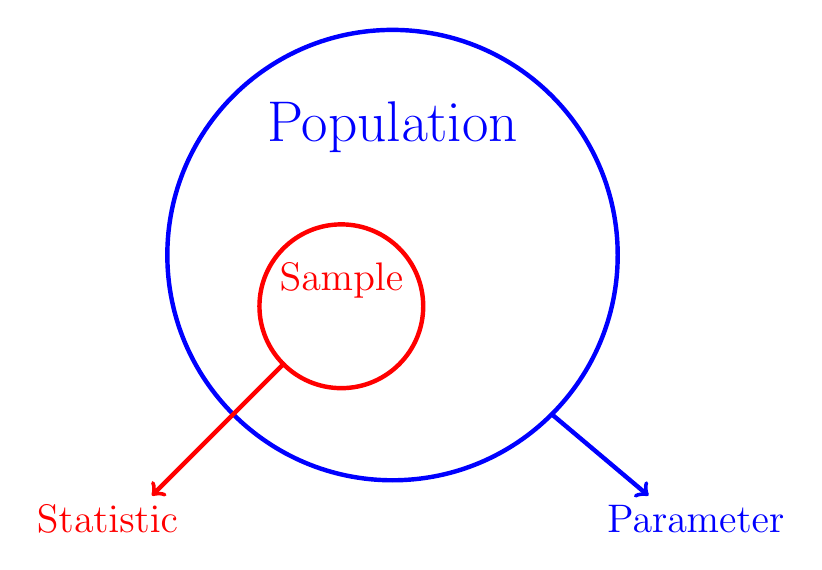
\begin{tikzpicture}[scale=1.3]
			\draw [blue, ultra thick] (0,0) circle [radius=2.2];
			\node [blue, font=\huge] at (0,1.25) {Population};
			\draw [blue, ultra thick, ->] (1.55,-1.55) -- (2.5,-2.35);
			\draw [red, ultra thick] (-0.5, -0.5) circle [radius=0.8];
			\node [blue, font =\Large, below right] at (2, -2.35) {Parameter};
			\node [red, font=\Large] at (-0.5, -0.25) {Sample};
			\draw [red, ultra thick, ->] (-1.05, -1.05) -- (-2.35, -2.35);
			\node [red, font =\Large, below left] at (-2, -2.35) {Statistic};
		\end{tikzpicture}
	\end{figure}
\end{frame}

%%%%%%%%%%%%%%%%%%%%%%%%%%%%%%%%%%%%%%%%
\begin{frame}
\frametitle{Kinds of Statistics}
	\begin{itemize}
		\item \textbf{Descriptive Statistics:} Graphical and numerical summaries of data
		\item \textbf{Inferential Statistics:} Using data to estimate, predict, and quantify 					uncertainty
	\end{itemize}
\end{frame}

%%%%%%%%%%%%%%%%%%%%%%%%%%%%%%%%%%%%%%%%
\begin{frame}
\frametitle{Why Do Statistics?}
	\begin{itemize}[<+- | alert@+>]
		\item \textbf{Ockham's Razor:} If we can predict everything based on the population, just 			get data on the population and call it a day, right? How hard can this really be?
		\item What's wrong with this reasoning?
		\begin{itemize}[<+- | alert@+>]
			\item \textbf{Limited resources:} Surveying the whole population is expensive and 					usually infeasible
			\item \textbf{Scarcity:} Sometimes only a small sample is available
			\item \textbf{Destructive testing:} Rating car parts for durability requires testing them 				until they break. If you tested every part, you'd have no parts to use in cars.
			\item \textbf{Error reduction:} Getting data on the whole population could aggravate 				measurement error if done improperly
		\end{itemize}
	\end{itemize}	
\end{frame}

%%%%%%%%%%%%%%%%%%%%%%%%%%%%%%%%%%%%%%%%
\begin{frame}
\frametitle{Sampling and Nonsampling Error}
In statistics we use samples to learn about populations, but samples almost never are \emph{exactly} like the population they are drawn from.
	\begin{enumerate}
		\item Sampling Error 
			\begin{itemize}
				\item \emph{Random} differences between sample and population
				\item Cancel out on average
				\item Decreases as sample size grows
			\end{itemize}
		\item Nonsampling Error
			\begin{itemize}
				\item \emph{Systematic} differences between sample and population 
				\item Does \emph{not} cancel out on average
				\item Does \emph{not} decrease as sample size grows
			\end{itemize}
	\end{enumerate}
\end{frame}

\section{Example: Historic Polling Mistake}
%%%%%%%%%%%%%%%%%%%%%%%%%%%%%%%%%%%%%%%%
\begin{frame}
\frametitle{Illustrative Example}
	\begin{center}
		\includegraphics[scale = 0.2]{./images/LiteraryDigest}
	\end{center}
\end{frame}

%%%%%%%%%%%%%%%%%%%%%%%%%%%%%%%%%%%%%%%%
\begin{frame}
\frametitle{Literary Digest -- 1936 Presidential Election Poll}
	\begin{center}
		\includegraphics[scale = 0.3]{./images/FDR}
		\includegraphics[scale = 1.67]{./images/Landon}\\
		\small{FDR versus Kansas Gov.\ Alf Landon}
	\end{center}

	\begin{block}{Data}
		Over 10 million ballots sent to those on auto registries and phone books. 
		
		2.4 million replied (Compared to  less than $45$ million votes cast in actual election)
	\end{block}
	
	\begin{block}{Prediction}
		Landslide for Landon: \emph{Landonslide},  if you will.
	\end{block}
\end{frame}

%%%%%%%%%%%%%%%%%%%%%%%%%%%%%%%%%%%%%%%%
\begin{frame}
\frametitle{What Could Go Wrong?}
	\begin{center}
		\includegraphics[scale = 0.3]{./images/FDR}
		\includegraphics[scale = 1.67]{./images/Landon}\\
		\small FDR versus Kansas Gov.\ Alf Landon
	\end{center}
	\normalsize
	\begin{center}
		\begin{tabular}{lcc}
									&Roosevelt		&Landon\\
		Literary Digest Prediction: 	&41\% 			& \alert{57\%}\\
		\onslide<3>{	Actual Result: 				&\alert{61\%} 	& 37\%}
		\end{tabular}
	\end{center}
	
	\onslide<2>{The rest is history. President Landon joined the ranks of forgettable presidents like 		Millard Fillmore and William Henry Harrison}
	\onslide<3>{\alert{\textbf{Oops}\ldots}}
\end{frame}

%%%%%%%%%%%%%%%%%%%%%%%%%%%%%%%%%%%%%%%%
\begin{frame}
\frametitle{What Went Wrong? \emph{Non-sampling Error (aka Bias)}}
	\begin{block}{Biased Sample}
		Sampled car owners and those with telephones
	\end{block}
	
	\begin{block}{Non-response Bias}
	Even if sample is unbiased, can't force people to reply.
		\begin{itemize}
			\item Among those who recieved a ballot, Landon supporters were more likely to reply.
		\end{itemize}
	\end{block}
	\alert{In this case, neither effect \emph{alone} was enough to throw off the result but together 		they did.}
	
	\tiny{Source: \href{http://www.jstor.org/stable/10.2307/2749114}{\fbox{Squire (1988)}}}
\end{frame}

%%%%%%%%%%%%%%%%%%%%%%%%%%%%%%%%%%%%%%%%
\begin{frame}
\frametitle{How Do You Get an Unbiased Sample?}
	\begin{block}{Simple Random Sample}	
		Each member of population is chosen strictly by chance, so that: (1) selection of one 					individual doesn't influence selection of any other, (2) each individual is just as likely to be 			chosen, (3) every possible sample of size $n$ has the same chance of selection.	
	\end{block}
	
	\begin{block}{What about non-response bias?}
	\end{block}
	
	\textbf{We'll cover how to quantify errors later in the course.}
\end{frame}

\section{Correlation, Causation, RCTs}
%%%%%%%%%%%%%%%%%%%%%%%%%%%%%%%%%%%%%%%%
\begin{frame}
\frametitle{Swimming Pools and Lead Poisoning}
	We asked a random sample of parents if they have an in-ground swimming pool and whether their child suffered from lead poisoning. We compare those who had pools to those who did not and find that those with pools had lower instances of lead poisoning. 
	\vspace{1em}
	Does this survey:
		\begin{enumerate}[(a)]
			\item Overstate health benefits of swimming (or really, having a swimming pool)
			\item Correctly identify health benefits of swimming
			\item Understate health benefits of swimming
			\item None of the above
		\end{enumerate}
\end{frame}

%%%%%%%%%%%%%%%%%%%%%%%%%%%%%%%%%%%%%%%%
\begin{frame}
\frametitle{Problem}
	Parents who own swimming pools may differ systematically from those who don't in 				\emph{other ways} that impact child's chance of getting lead poisoning!
	\vspace{2em}
	\begin{alertblock}{Wealth influences one's ability to have a swimming pool and to live in a house without lead paint.}
	\end{alertblock}
\end{frame}

%%%%%%%%%%%%%%%%%%%%%%%%%%%%%%%%%%%%%%%%
\begin{frame}
\frametitle{Confounder}
	Factor than influences both outcomes and whether subjects are treated or not. Masks true 			effect of treatment.
\end{frame}

%%%%%%%%%%%%%%%%%%%%%%%%%%%%%%%%%%%%%%%%
\begin{frame}
\frametitle{Properly Determining Treatment Effectiveness: Randomized Experiments}
	\begin{itemize}
		\item Start with group of experimental subjects
		\item Randomly assign one group to get the ``treatment'' and the other gets nothing (i.e. the ``control'' group)
		\item Random assignment neutralizes the chance of confounding factors since groups are 			initially equal, on average, and only difference is the treatment.
	\end{itemize}
	\alert{Double-blind randomized trials are the gold standard}
\end{frame}

%%%%%%%%%%%%%%%%%%%%%%%%%%%%%%%%%%%%%%%%
\begin{frame}
\frametitle{Double-Blind Randomized Trial}
\begin{figure}
\centering
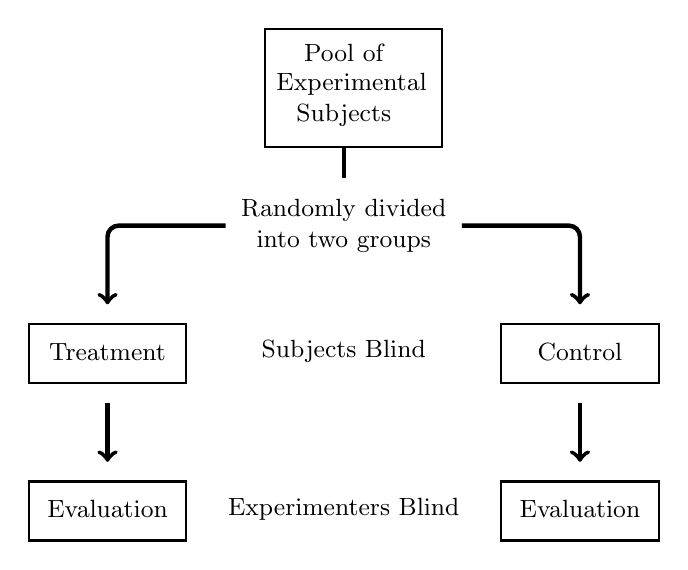
\begin{tikzpicture}
	\draw [thick] (0,0) rectangle (2.25,1.5);
	\draw [ultra thick] (1,0) -- (1,-0.4);
	\draw [ultra thick, ->, rounded corners] (2.5,-1) -- (4,-1) -- (4, -2);
	\draw [ultra thick, ->, rounded corners] (-0.5,-1) -- (-2,-1) -- (-2, -2);
	\draw [ultra thick, ->] (-2, -3.25) -- (-2, -4); 
	\draw [ultra thick, ->] (4, -3.25) -- (4, -4); 
	\draw [thick] (3,-2.25) rectangle (5,-3);
	\draw [thick] (3,-4.25) rectangle (5,-5);
	\draw [thick] (-3,-2.25) rectangle (-1,-3);
	\draw [thick] (-3,-4.25) rectangle (-1,-5);
	\node [font=\small] at (1,1.2) {Pool of};
	\node [font=\small] at (1.1,0.8) {Experimental};
	\node [font=\small] at (1,0.4) {Subjects};
	\node [font=\small] at (1,-0.8) {Randomly divided};
	\node [font=\small] at (1,-1.2) {into two groups};
	\node [font=\small] at (1,-2.6) {Subjects Blind};
	\node [font=\small] at (1,-4.6) {Experimenters Blind};
	\node [font=\small] at (4,-2.6) {Control};
	\node [font=\small] at (4,-4.6) {Evaluation};
	\node [font=\small] at (-2,-2.6) {Treatment};
	\node [font=\small] at (-2,-4.6) {Evaluation};
\end{tikzpicture}
\end{figure}
\end{frame}

%%%%%%%%%%%%%%%%%%%%%%%%%%%%%%%%%%%%%%%%
\begin{frame}
\frametitle{Gold Standard: Randomized, Double-blind Experiment}
	\begin{quote}
		Randomized blind experiments ensure that on average the two groups are initially equal, and continue to be treated equally. Thus a fair comparison is possible.
	\end{quote}
	
	\vspace{2em}
	\begin{alertblock}{Randomized, double-blind experiments are generally the best way to untangle causation.}
	\end{alertblock}
\end{frame}

%%%%%%%%%%%%%%%%%%%%%%%%%%%%%%%%%%%%%%%%
\begin{frame}
\frametitle{Randomized Trials and Real Life}
	\begin{itemize}[<+- | alert@+>]
		\item \alert{Ockham's Razor II:} Randomize everything and fix this whole causation/correlation problem!
		\item What Shall We Solve?
			\begin{itemize}
				\item Does gender affect one's wages?
				\item Does the defendant's race affect their sentencing?
				\item Does spanking cause criminality?
			\end{itemize}
		\end{itemize}
\end{frame}

%%%%%%%%%%%%%%%%%%%%%%%%%%%%%%%%%%%%%%%%
\begin{frame}
	\Huge{Randomization is not always possible, practical, or ethical.}
\end{frame}

%%%%%%%%%%%%%%%%%%%%%%%%%%%%%%%%%%%%%%%%
\begin{frame}
	\frametitle{Aperture Science and Randomized Trials}
	\begin{center}
		\includegraphics[scale=1]{./images/aperture.png}
	\end{center}
	\href{run:./sound/Cave_Johnson_mandatory_testing.wav}{\beamergotobutton{Mandatory Testing}}
	\href{run:./sound/Cave_Johnson_control1.wav}{\beamergotobutton{Control Groups}}
	\href{run:./sound/Cave_Johnson_control2.wav}{\beamergotobutton{Control Groups (ct'd)}}
\end{frame}

%%%%%%%%%%%%%%%%%%%%%%%%%%%%%%%%%%%%%%%%
\begin{frame}
\frametitle{How Can We Learn Anything Without Randomized Experiments?}
	\begin{block}{Observational Data}
		Data that do not come from a randomized experiment.	
	\end{block}
	\vspace{2em}
	\begin{alertblock}{It is very difficult to untangle cause and effect using observational data because of confounders.}
	\end{alertblock}
\end{frame}

%%%%%%%%%%%%%%%%%%%%%%%%%%%%%%%%%%%%%%%%
\begin{frame}
\frametitle{Does Racial Discrimination  Affect Criminal Sentencing?}
	\begin{quote}
	\footnotesize
		Social scientists have studied the issue for decades, but the seemingly simple question ``Does race affect sentencing?'' is surprisingly difficult to answer on the basis of empirical evidence.
		
		Abrams explains: \alert{``The most straightforward way you might look at it is to say, Let’s look at what sentences people get and see whether sentence length varies by race. If it looks like people of one race receive longer sentences than another, that might indicate that the criminal justice system is unfair. But the shortcoming to that approach is that it’s also possible that sentences can differ for many reasons; for example, it’s possible people of different races might have different criminal histories on average, and that could also explain the difference in sentence length.''}
	\end{quote}
	\tiny{Source: \href{https://www.law.upenn.edu/live/news/2170-new-study-by-professor-david-s-abrams-confirms}{\fbox{Penn Law Website}}}
\end{frame}

%%%%%%%%%%%%%%%%%%%%%%%%%%%%%%%%%%%%%%%%
\begin{frame}
\frametitle{Reducing Bias in Observational Studies}
	\begin{block}{Regression}
	Technique that allows us to remove influence of confounders. Works well if we can identify and gather data on all of them. But...
	\end{block}
\end{frame}

%%%%%%%%%%%%%%%%%%%%%%%%%%%%%%%%%%%%%%%%
\begin{frame}
\frametitle{Does Racial Discrimination  Affect Criminal Sentencing?}
	\footnotesize
	\begin{quote}
		To address that difficulty [confounders] social scientists have ... applied control variables to standard regression equations, a statistical method for identifying significant correlations between observed events. For instance, controlling for type of crime committed or for the defendant’s criminal history, researchers look to see whether the results of their equation still show racial disparity.\alert{``The problem with that is you still leave the possibility that any differences you see are due to unobserved variables, differences that might be there but that you can't control for''} Abrams says.``That might be demeanor in the courtroom, it might be the quality of the attorney you can afford, it might be some details about the crime that you might not capture in your data. If those things are correlated with race, which they probably are, you're not going to know whether the effect you think you're detecting is really race or is something else.''
	\end{quote}
	
	\tiny{Source: \href{https://www.law.upenn.edu/live/news/2170-new-study-by-professor-david-s-abrams-confirms}{\fbox{Penn Law Website}}}
\end{frame}

%%%%%%%%%%%%%%%%%%%%%%%%%%%%%%%%%%%%%%%%
\begin{frame}
\frametitle{Related Reading}
	\begin{itemize}
		\item Wonnacott: Chapter 1
		\item How to Lie with Statistics: Chapter 1
	\end{itemize}
\end{frame}

%%%%%%%%%%%%%%%%%%%%%%%%%%%%%%%%%%%%%%%%
\begin{frame}
\frametitle{Homework}
	\begin{itemize}
		\item Math diagnostic
		\item Chapter 1 Problems
		\item R Tutorial 1
	\end{itemize}
\end{frame}

%%%%%%%%%%%%%%%%%%%%%%%%%%%%%%%%%%%%%%%%
\end{document}
